% SWAMPE-JAX paper, typeset in the Journal of Open Source Software (JOSS) format.
% Reproduces the Open Journals LaTeX template (left metadata sidebar, logo header,
% CC-BY footer). Build with:  make   (pdflatex -> bibtex -> pdflatex x2)
\documentclass[10pt,a4paper,onecolumn]{article}
\usepackage{graphicx}
\usepackage{xcolor}
\usepackage{etoolbox}
\usepackage{titlesec}
\usepackage{calc}
\usepackage{tikz}
\usepackage{hyperref}
\hypersetup{colorlinks,breaklinks=true,
            urlcolor=[rgb]{0.0, 0.5, 1.0},
            linkcolor=[rgb]{0.0, 0.5, 1.0}}
\usepackage{caption}
\usepackage{tcolorbox}
\usepackage{amssymb,amsmath}
\usepackage{ifxetex,ifluatex}
\usepackage{xstring}

% seqsplit is unavailable here; \seqsplit only governs long-string line breaking,
% so we shim it to a no-op and keep \texttt unmodified.
\providecommand{\seqsplit}[1]{#1}
\let\textttOrig=\texttt

% Force figures to stay in place (JOSS template behaviour).
\usepackage{float}
\let\origfigure\figure
\let\endorigfigure\endfigure
\renewenvironment{figure}[1][2] {
    \expandafter\origfigure\expandafter[H]
} {
    \endorigfigure
}

% --- Bibliography: natbib + bibtex (biber/biblatex unavailable here) ----------
\usepackage[round]{natbib}
\bibliographystyle{plainnat}

% --- DOI-aware link splitting (uses xstring) ---------------------------------
\makeatletter
\let\href@Orig=\href
\def\href@Urllike#1#2{\href@Orig{#1}{\begingroup
    \def\Url@String{#2}\Url@FormatString
    \endgroup}}
\def\href@Notdoi#1#2{\def\tempa{#1}\def\tempb{#2}%
  \ifx\tempa\tempb\relax\href@Urllike{#1}{#2}\else
  \href@Orig{#1}{#2}\fi}
\def\href#1#2{%
  \IfBeginWith{#1}{https://doi.org}%
  {\href@Urllike{#1}{#2}}{\href@Notdoi{#1}{#2}}}
\makeatother

% --- Page layout: left metadata margin (reversemp) ---------------------------
\usepackage[top=3.5cm, bottom=3cm, right=1.5cm, left=1.0cm,
            headheight=2.2cm, reversemp, includemp, marginparwidth=4.5cm]{geometry}

% --- Default font ------------------------------------------------------------
\renewcommand\familydefault{\sfdefault}

% --- Style -------------------------------------------------------------------
\renewcommand{\bibfont}{\small \sffamily}
\renewcommand{\captionfont}{\small\sffamily}
\renewcommand{\captionlabelfont}{\bfseries}

% --- Section/SubSection/SubSubSection ----------------------------------------
\titleformat{\section}
  {\normalfont\sffamily\Large\bfseries}
  {}{0pt}{}
\titleformat{\subsection}
  {\normalfont\sffamily\large\bfseries}
  {}{0pt}{}
\titleformat{\subsubsection}
  {\normalfont\sffamily\bfseries}
  {}{0pt}{}
\titleformat*{\paragraph}
  {\sffamily\normalsize\bfseries}

% --- Header / Footer ---------------------------------------------------------
\usepackage{fancyhdr}
\pagestyle{fancy}
\fancyhf{}
\renewcommand{\headrulewidth}{0pt}
\fancyhead[L]{\hspace{-0.75cm}
\includegraphics[width=5.5cm]{joss-logo.png}}
\fancyhead[C]{}
\fancyhead[R]{}
\renewcommand{\footrulewidth}{0.25pt}

\fancyfoot[L]{\parbox[t]{0.98\headwidth}{\footnotesize{\sffamily Malsky et al. (2026). SWAMPE-JAX: A differentiable JAX implementation of the SWAMPE shallow-water model for exoplanet atmospheres. \textit{Journal of Open Source Software}, X(XX), XXXX. \url{https://doi.org/10.21105/joss.0XXXX}}}}

\fancyfoot[R]{\sffamily \thepage}
\makeatletter
\let\ps@plain\ps@fancy
\fancyheadoffset[L]{4.5cm}
\fancyfootoffset[L]{4.5cm}

% --- Macros ------------------------------------------------------------------
\definecolor{linky}{rgb}{0.0, 0.5, 1.0}
\definecolor{orcidlogocol}{HTML}{A6CE39}
% Lightweight ORCID iD icon (orcidlink.sty is unavailable in this TeX install).
\newcommand{\orcid}[1]{\href{https://orcid.org/#1}{\mbox{\tikz[baseline=-0.55ex]%
  \node[circle,fill=orcidlogocol,inner sep=1pt]{\textcolor{white}{\tiny\bfseries iD}};}}}

\newcommand{\ExternalLink}{%
   \tikz[x=1.2ex, y=1.2ex, baseline=-0.05ex]{%
       \begin{scope}[x=1ex, y=1ex]
           \clip (-0.1,-0.1)
               --++ (-0, 1.2)
               --++ (0.6, 0)
               --++ (0, -0.6)
               --++ (0.6, 0)
               --++ (0, -1);
           \path[draw,
               line width = 0.5,
               rounded corners=0.5]
               (0,0) rectangle (1,1);
       \end{scope}
       \path[draw, line width = 0.5] (0.5, 0.5)
           -- (1, 1);
       \path[draw, line width = 0.5] (0.6, 1)
           -- (1, 1) -- (1, 0.6);
       }
   }

% --- Title / Authors (flush left, per JOSS template; authblk-free) -----------
\makeatletter
\patchcmd{\@maketitle}{center}{flushleft}{}{}
\patchcmd{\@maketitle}{center}{flushleft}{}{}
\patchcmd{\@maketitle}{\LARGE}{\LARGE\sffamily}{}{}
\renewcommand{\maketitle}{{%
  \renewenvironment{tabular}[2][]{\begin{flushleft}}{\end{flushleft}}%
  \@maketitle}}
\makeatother

\usepackage[T1]{fontenc}
\usepackage[utf8]{inputenc}
\IfFileExists{microtype.sty}{\usepackage{microtype}}{}

\IfFileExists{parskip.sty}{\usepackage{parskip}}{%
\setlength{\parindent}{0pt}
\setlength{\parskip}{6pt plus 2pt minus 1pt}}
\setlength{\emergencystretch}{3em}
\providecommand{\tightlist}{\setlength{\itemsep}{0pt}\setlength{\parskip}{0pt}}
\setcounter{secnumdepth}{0}

% --- Title block -------------------------------------------------------------
\title{SWAMPE-JAX: A differentiable JAX implementation of the SWAMPE
       shallow-water model for exoplanet atmospheres}

\author{%
  \bfseries
  Isaac Malsky\,\orcid{0000-0003-0217-3880}$^{1}$,\enspace
  Shreyas Vissapragada\,\orcid{0000-0003-4015-9975}$^{2}$,\enspace
  Ekaterina Landgren\,\orcid{0000-0001-6029-5216}$^{3}$\\[0.6em]
  \normalsize\mdseries
  $^{1}$Jet Propulsion Laboratory, California Institute of Technology, Pasadena, CA 91109, USA\\
  $^{2}$The Observatories of the Carnegie Institution for Science, Pasadena, CA 91101, USA\\
  $^{3}$Cooperative Institute for Research in Environmental Sciences, University of Colorado Boulder, Boulder, CO 80309, USA}
\date{\vspace{-7ex}}

\begin{document}
\maketitle

% --- Left metadata sidebar ---------------------------------------------------
\marginpar{

  \begin{flushleft}
  \sffamily\small

  {\bfseries DOI:} \href{https://doi.org/10.21105/joss.0XXXX}{\color{linky}{10.21105/joss.0XXXX}}

  \vspace{2mm}

  {\bfseries Software}
  \begin{itemize}
    \setlength\itemsep{0em}
    \item \href{https://github.com/openjournals/joss-reviews/issues/XXXX}{\color{linky}{Review}} \ExternalLink
    \item \href{https://github.com/imalsky/MY_SWAMP}{\color{linky}{Repository}} \ExternalLink
    \item \href{https://doi.org/10.5281/zenodo.XXXXXXX}{\color{linky}{Archive}} \ExternalLink
  \end{itemize}

  \vspace{2mm}

  \par\noindent\hrulefill\par

  \vspace{2mm}

  {\bfseries Editor:} Pending \ExternalLink \\
  \vspace{1mm}
  {\bfseries Reviewers:}
  \begin{itemize}
  \setlength\itemsep{0em}
  \item Pending
  \end{itemize}
  \vspace{2mm}

  {\bfseries Submitted:} 24 June 2026\\
  {\bfseries Published:} Pending

  \vspace{2mm}
  {\bfseries License}\\
  Authors of papers retain copyright and release the work under a Creative Commons Attribution 4.0 International License (\href{http://creativecommons.org/licenses/by/4.0/}{\color{linky}{CC BY 4.0}}).

  \end{flushleft}
}

% =============================================================================
\section{Summary}

The vast majority of exoplanets with measurable atmospheres are spin-synchronized:
one hemisphere is constantly irradiated, and the other sees eternal night. This
permanent imbalance in thermal forcing, coupled with rotation, makes the
atmospheres we can characterize inherently multidimensional \citep{Showman:2009,
Kataria:2016}. Because exoplanets are observed almost entirely through indirect,
disk-integrated measurements, recovering this structure rests on atmospheric
models. One-dimensional models are fast and sweep large parameter ranges but
cannot represent variation with longitude; three-dimensional general circulation
models resolve the full circulation but at a computational cost that makes wide
parameter studies expensive. Two-dimensional shallow-water models fill the gap:
they capture the day--night circulation and equatorial jets of close-in planets
while remaining cheap enough to explore parameter space and isolate the dynamical
mechanisms at work.

\texttt{SWAMPE-JAX} (installed and imported as \texttt{my\_swamp}) is a Python
package for modeling the two-dimensional dynamics of exoplanet atmospheres. It
solves the shallow-water equations on the rotating sphere using the
spectral-transform method, advancing absolute vorticity, divergence, and
geopotential forward in time, and is benchmarked for synchronously rotating hot
Jupiters and sub-Neptunes. \texttt{SWAMPE-JAX} is a \texttt{JAX} \citep{jax:2018}
reimplementation of \texttt{SWAMPE} \citep{Landgren:2022}, which it reproduces to
high precision. Its new capability is differentiability: the simulated
geopotential and wind fields, and any quantity derived from them, can be
differentiated with respect to the planet's physical parameters and initial
conditions through automatic differentiation. The same code is just-in-time
compiled, runs on CPU or GPU, and can be vectorized over batches of parameters in
a single call. These gradients give the exact sensitivity of the simulated
atmosphere to the forcing mechanisms and timescales that shape it, at a cost
comparable to a single forward run.

\section{Statement of need}

Interpreting these atmospheres requires forward models, and existing ones force a
choice between speed and physical fidelity. One-dimensional radiative--convective
models are cheap and retain vertical thermal structure but cannot resolve
variation with longitude, and so cannot self-consistently link the forcing to the
day--night circulation that shapes the data. Three-dimensional general circulation models
\citep[e.g.,][]{Showman:2009, Kataria:2016, Carone:2020} capture the full spatial
structure but are far too expensive to explore widely: converging one deep
hot-Jupiter model costs tens of thousands of CPU-hours \citep{Roth:2024}, and a
single sub-Neptune takes months of wall-clock time \citep{Wang:2020}. There is a pressing need for a multidimensional forward model
fast enough to sweep parameter space and isolate the causal drivers that shape
exoplanet atmospheres.

Two-dimensional shallow-water models occupy this middle ground. By representing
the atmosphere as a single active layer, they trade away vertical structure but
capture the day--night circulation \citep{Perez-Becker:2013}, equatorial
superrotation \citep{Showman:2011}, and, in some regimes, atmospheric
time-variability \citep{Menou:2003}, while remaining cheap enough to sweep
parameter space and to isolate how the radiative and drag timescales set the
balance between external forcing and atmospheric transport \citep{Komacek:2016}.
The framework is not restricted to synchronous rotation, since the rotation rate
is a free parameter; tidal locking enters only through the standard day--night
Newtonian-relaxation forcing, which fixes the radiative-equilibrium hot spot to a
permanent substellar point (the fixed-substellar idealization of
\citealt{Landgren:2023}). \texttt{SWAMPE} made this class of model openly
available and well documented in Python \citep{Landgren:2022, Landgren:2023}.

Isolating these drivers, however, requires not just fast forward simulations but
their derivatives. Sensitivity analysis and gradient-based parameter studies both
depend on how the simulated state responds to the underlying physical controls:
the radiative and drag timescales, the day--night forcing amplitude, the reference
geopotential, and the rotation rate. Obtaining these derivatives from a
traditional NumPy model means perturbing each parameter, rerunning, and
differencing the results, at a cost of one forward run per parameter and with
finite-difference noise. \texttt{SWAMPE-JAX} removes this bottleneck: because the
solver is written in \texttt{JAX}, automatic differentiation applies the chain
rule across the entire time integration and returns exact gradients at a cost
comparable to a single forward run, independent of the number of parameters. The
same gradients resolve how each region of the simulated atmosphere responds to the
forcing timescales (\autoref{fig:sensitivity}), turning a finite-difference loop
whose cost grows with the number of parameters into a single differentiation.

\section{Functionality}

\texttt{SWAMPE-JAX} preserves the public interface and the numerical behavior of
\texttt{SWAMPE}, so that existing workflows port with minimal changes, while
adding the capabilities that \texttt{JAX} makes possible:

\begin{itemize}
\item \textbf{Differentiability.} The time-stepping loop runs inside
  \texttt{jax.lax.scan}, which makes the terminal state and any scalar loss
  differentiable with respect to the continuous physical parameters (day--night
  forcing contrast, radiative and drag timescales, mean geopotential, rotation
  rate, planetary radius, timestep, and hyperdiffusion coefficients) and with
  respect to explicit initial conditions. Reverse-mode gradients
  (\texttt{jax.grad}) are validated against centered finite differences;
  forward-mode differentiation (\texttt{jax.jvp}, \texttt{jax.jacfwd}) is also
  supported. Because reverse-mode cost is independent of the number of
  parameters, we find that the gradient of a scalar loss with respect to four
  physical parameters costs about $2.0\times$ a single forward integration
  (measured at spectral truncation $M=42$ on an Apple~M3~Pro: a ten-day forced run
  takes $18.0$~s and its gradient $36.1$~s, after one-time compilation), compared
  with the five forward integrations a one-sided finite-difference gradient over
  the same four parameters would require. \autoref{fig:sensitivity} illustrates the payoff: a single
  differentiation maps how the simulated temperature field responds, point by
  point, to the radiative and drag forcing timescales over a $100$-day forced
  hot-Jupiter integration.
\item \textbf{Acceleration and vectorization.} The same code is just-in-time
  compiled with \texttt{jax.jit} and runs unchanged on CPU or GPU. A ten-day,
  $M=42$ forced integration that takes about $14.5$~minutes ($871$~s) in reference
  NumPy \texttt{SWAMPE} completes in about $29$~seconds in \texttt{SWAMPE-JAX} on
  the same machine, including one-time compilation, a roughly $30\times$ speedup
  (measured on an Apple~M3~Pro, \texttt{JAX}~0.9.2). \texttt{jax.vmap} maps the
  simulator over batches of parameters in a single compiled call, enabling large
  ensemble parameter sweeps.
\item \textbf{Numerical parity.} For default settings, \texttt{SWAMPE-JAX}
  reproduces \texttt{SWAMPE}'s spectral-transform solver \citep{Hack:1992},
  modified-Euler time differencing \citep{Langton:2008}, Robert--Asselin
  filtering, sixth-order hyperdiffusion \citep{Gelb:2001}, and
  Newtonian-relaxation-plus-drag forcing, including the historical conventions of
  the reference code. Agreement is not bit-exact, because XLA and NumPy do not
  evaluate floating-point expressions in the same order, but over a ten-day
  forced hot-Jupiter integration the two implementations agree to a fractional
  difference below $2\times10^{-7}$ in every field, with the geopotential
  matching to a few parts in $10^{10}$ (\autoref{fig:parity}); the automated test
  suite enforces tighter absolute tolerances still ($10^{-10}$ for vorticity and
  divergence, $5\times10^{-8}$ for geopotential).
\end{itemize}

Together, these features let \texttt{SWAMPE-JAX} serve both as a drop-in
replacement for \texttt{SWAMPE} and as a differentiable forward model for
sensitivity analysis and gradient-based parameter studies.

\begin{figure}[t]
\centering
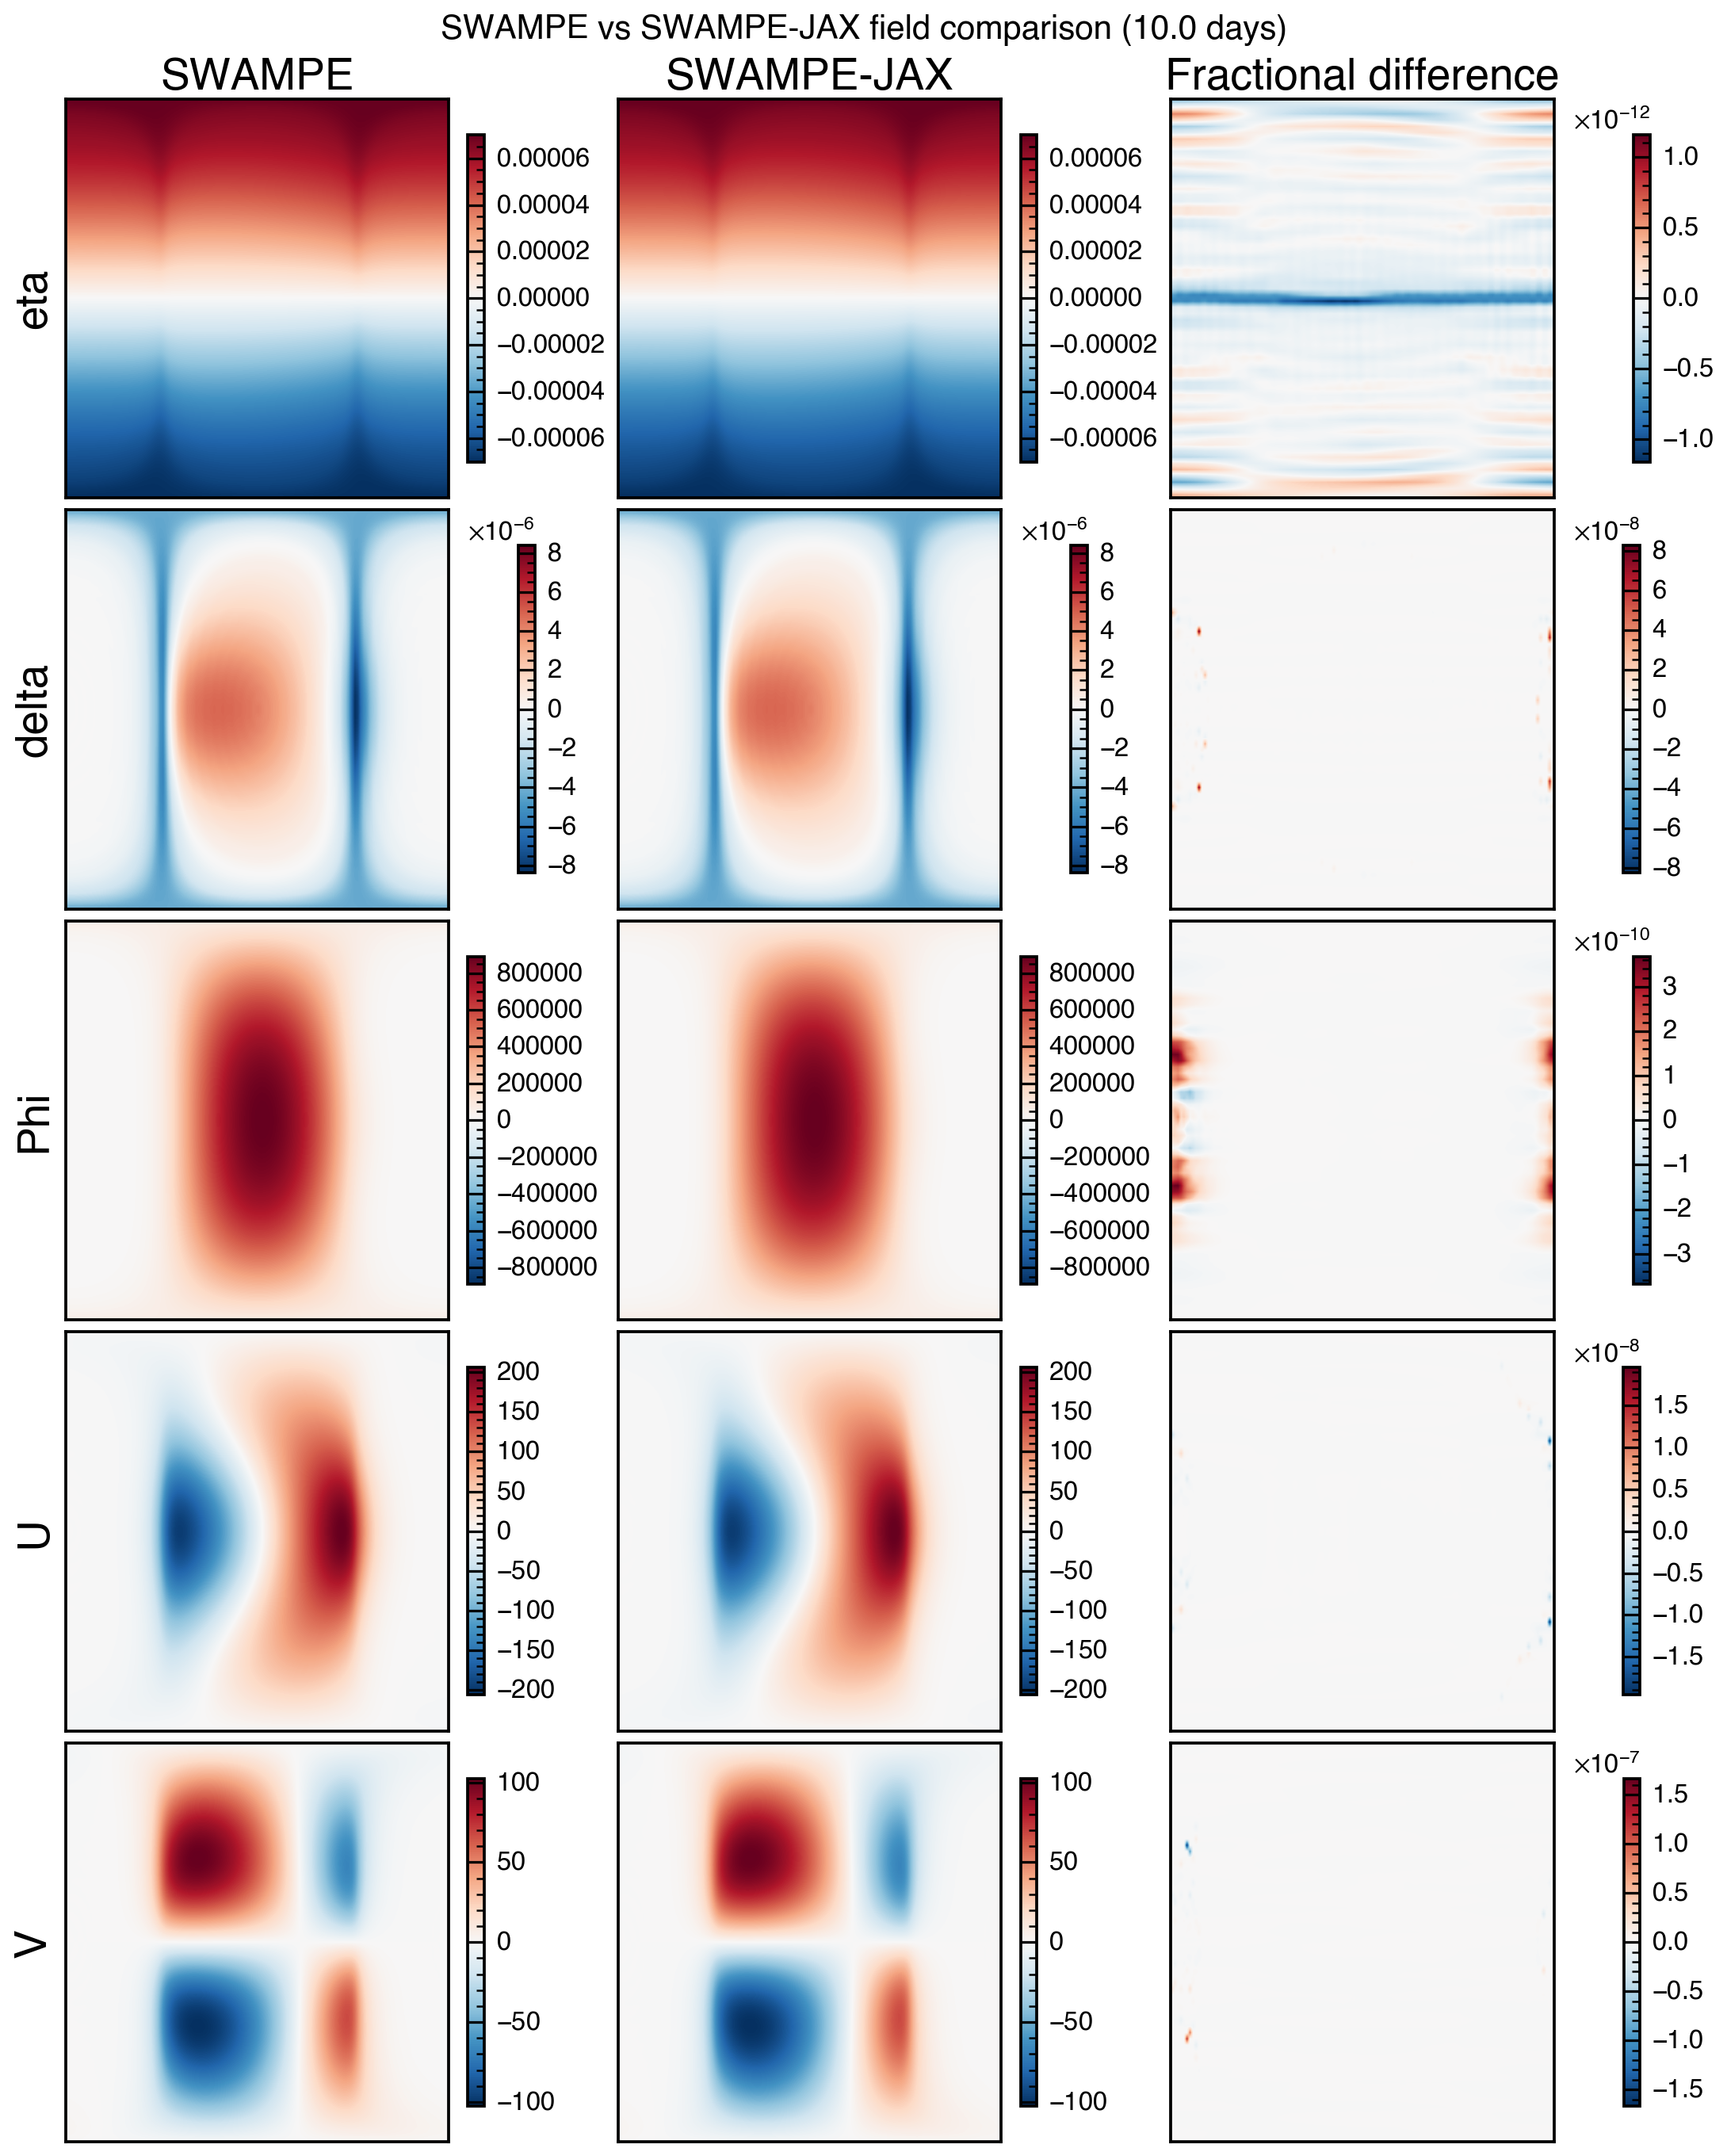
\includegraphics[width=\linewidth]{parity_comparison.png}
\caption{Numerical parity between reference NumPy \texttt{SWAMPE} (left column)
and \texttt{SWAMPE-JAX} (middle column) for a forced hot-Jupiter integration. A
day--night Newtonian-relaxation forcing (amplitude
$\Delta\Phi_{\mathrm{eq}}=10^{6}\,\mathrm{m^2\,s^{-2}}$, radiative and drag
timescales of $10$ and $6$~hours) acts on a synchronously rotating planet with
mean geopotential $\overline{\Phi}=3\times10^{5}\,\mathrm{m^2\,s^{-2}}$, rotation
rate $\Omega=3.2\times10^{-5}\,\mathrm{s^{-1}}$, and radius
$a=8.2\times10^{7}$~m, integrated for ten days at spectral truncation $M=42$ with
a timestep of $120$~s. The forcing produces a hot substellar geopotential bulge
and a superrotating equatorial jet; the total geopotential
$\overline{\Phi}+\Phi$ stays positive everywhere, so the shallow-water layer
thickness remains well defined. Rows show the absolute vorticity $\eta$,
divergence $\delta$, geopotential $\Phi$, and the zonal and meridional winds $U$
and $V$; the right column is the signed fractional difference between the two
codes. Agreement is everywhere better than a fractional difference of
$2\times10^{-7}$: the geopotential matches to a few parts in $10^{10}$ and the
winds to better than two parts in $10^{7}$.}
\label{fig:parity}
\end{figure}

\begin{figure}[t]
\centering
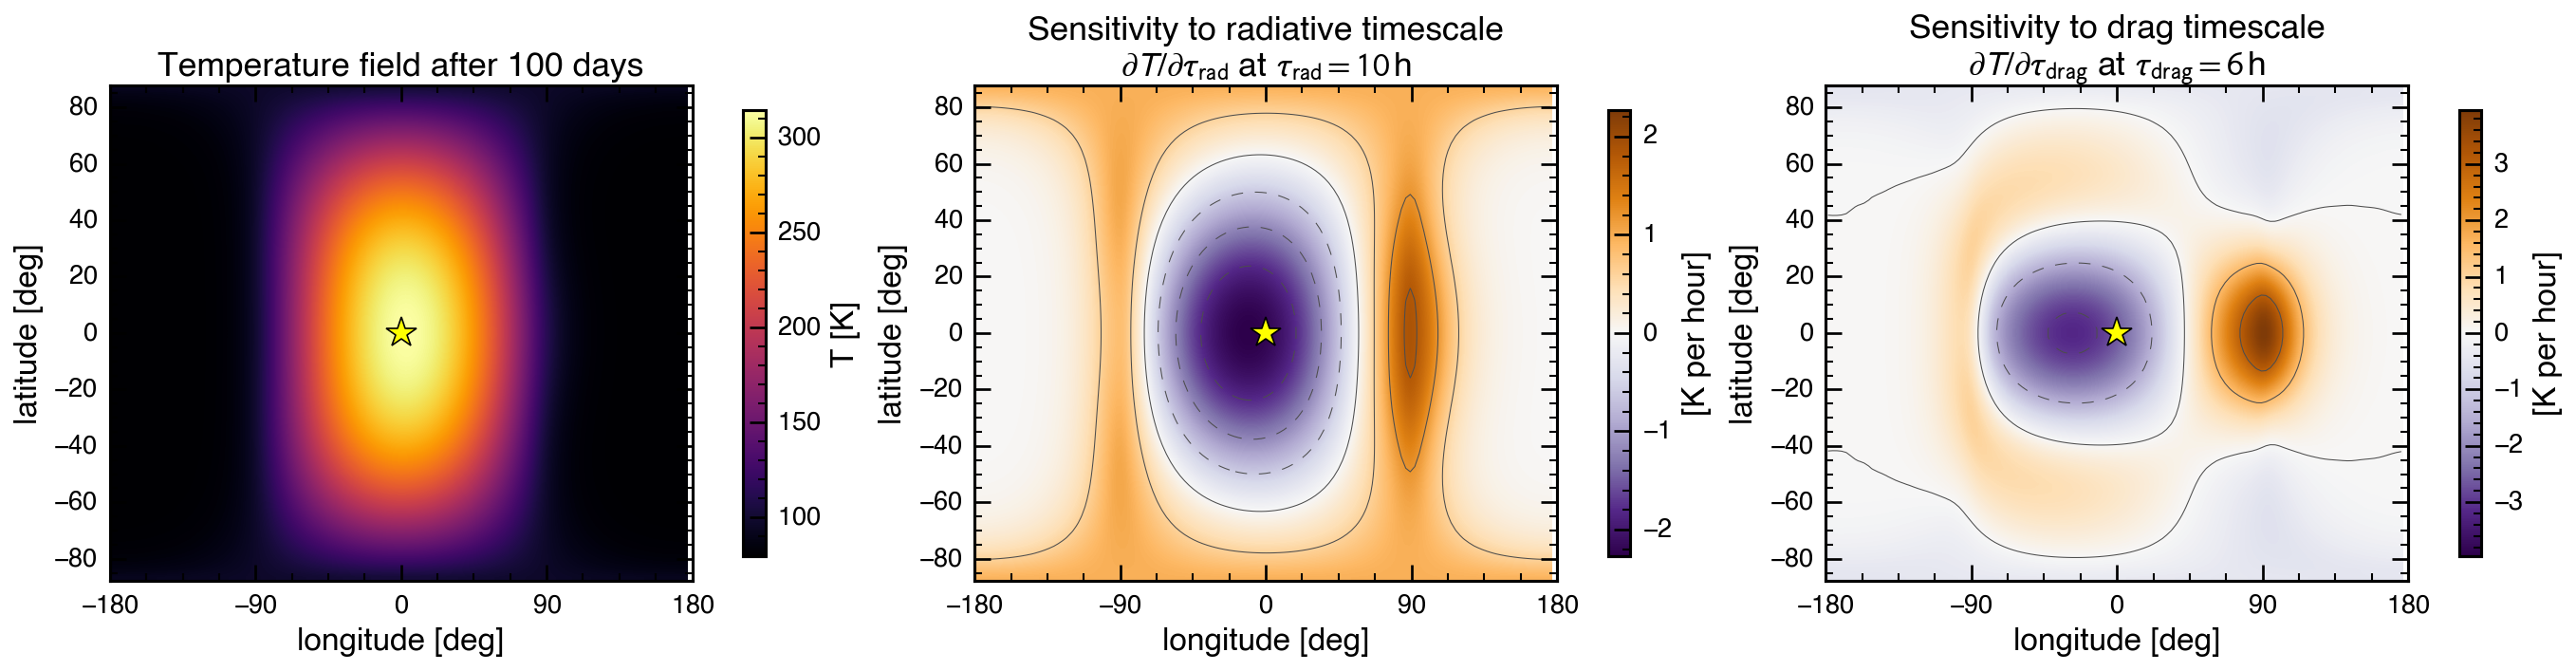
\includegraphics[width=\linewidth]{temperature_sensitivity_perhour_100d.png}
\caption{Spatially resolved sensitivities of a forced hot-Jupiter atmosphere,
obtained by automatic differentiation through a $100$-day integration in the
regime of \autoref{fig:parity} (spectral truncation $M=42$, radiative timescale
$\tau_{\mathrm{rad}}=10$~h, drag timescale $\tau_{\mathrm{drag}}=6$~h). From left
to right, the panels show the simulated temperature field (a shallow-water proxy
$T=(\overline{\Phi}+\Phi)/R_d$ with $R_d=3.78\times10^{3}\,\mathrm{J\,kg^{-1}\,K^{-1}}$;
the substellar point is marked) and the exact derivative of that field with
respect to the radiative timescale, $\partial T/\partial\tau_{\mathrm{rad}}$, and
the drag timescale, $\partial T/\partial\tau_{\mathrm{drag}}$, both in K per hour.
Each map is obtained from a single forward-mode pass through the full time
integration, with no additional forward runs, and reproduces a finite-difference
response to $r^2=0.998$ and $r^2=0.985$ for the radiative and drag panels
respectively. Both sensitivities are largest near the substellar
point: $\partial T/\partial\tau_{\mathrm{rad}}$ peaks on the hot spot itself and
$\partial T/\partial\tau_{\mathrm{drag}}$ just downwind of it, decaying across the
quiet nightside. Lengthening either timescale erodes the day--night contrast, the
radiative timescale by weakening the thermal forcing and the drag timescale by
letting the stronger circulation redistribute more heat.}
\label{fig:sensitivity}
\end{figure}

\section{Relation to SWAMPE and similar tools}

\texttt{SWAMPE-JAX} shares an interface and a set of physical benchmarks with
\texttt{SWAMPE} \citep{Landgren:2022} but no source code; it is not a wrapper.
Reduced and two-dimensional dynamical models have a long history in exoplanet
science: barotropic and shallow-water treatments of close-in giant planets
\citep{Cho:2008}, analytic shallow-water theories of the day--night flow
\citep{HengWorkman:2014}, and linear and diagnostic models of the wave-driven
circulation \citep{Showman:2011, Hammond:2021}. \texttt{SWAMPE-JAX} adds
automatic differentiation and GPU execution to this family. Differentiable,
GPU-capable simulation has advanced neighboring fields, including
machine-learning-accelerated computational fluid dynamics \citep{Kochkov:2021},
neural general circulation models for Earth weather and climate
\citep{Kochkov:2024}, and general spectral frameworks such as Dedalus
\citep{Burns:2020}. Within exoplanet science, \texttt{ExoJAX}
\citep{Kawahara:2022} brought automatic differentiation to high-resolution
radiative transfer and spectral retrieval; \texttt{SWAMPE-JAX} is complementary
in that it makes the atmospheric \textit{dynamics} differentiable. To our
knowledge, no openly available exoplanet shallow-water model exposes gradients
through the full atmospheric integration, and \texttt{SWAMPE-JAX} fills that gap
while retaining the validated physics of \texttt{SWAMPE}.

\section{Acknowledgements}

We thank Alice Nadeau for co-developing and openly releasing the original
\texttt{SWAMPE} model. The authors used Claude (Anthropic) to assist with code
development, code cleanup, and manuscript preparation. We acknowledge the
developers of the open-source packages on which this work depends, in particular
\texttt{JAX} \citep{jax:2018}, \texttt{NumPy} \citep{Harris:2020}, \texttt{SciPy}
\citep{Virtanen:2020}, and \texttt{Matplotlib} \citep{Hunter:2007}.

\bibliography{paper}

\end{document}
